\section{Analysis 3: Supplementary Results}

\paragraph{Language representations.} Figure~\ref{fig:a3-spatial} gives the spatial-term rate for every norm category, Figure~\ref{fig:a3-probe} compares the three representations, and Figure~\ref{fig:a3-tsne} shows the t-SNE, in which categories overlap rather than form clusters. A six-way probe on the primary category reaches 46.3\% [44.0, 48.7] with BERT and 33.9\% [31.7, 36.1] with Empath (majority 25.5\%; $n{=}1{,}794$ correct options that carry a category label). A BERT probe over option text alone selects the labelled option on 58.7\% [56.5, 61.0] of the 1{,}832 items whose labelled answer is a real option (chance 25\%; Empath 44.7\%). Length is not the cue: choosing the longest option gives 22.1\%, and correct and distractor options average 22.2 and 22.8 words. The spatial lexicon is coarse (\emph{way}, \emph{clear}, \emph{close} have non-spatial senses), so its rates are upper bounds.

\paragraph{Sixty-item protocol.} The verified split has 200 items from 183 source videos. We keep one item per video in a fixed hash order, sample five frames at 10, 30, 50, 70 and 90\% of the pre-action clip, and rank items by the minimum Laplacian variance over the five frames; the 60 sharpest are used (minimum variance 895--5{,}220, against a median of 286 for the other 123). Action and justification options are permuted per item with a fixed seed. The prompt text is the same for every model and tells it not to answer ``none of these'', which is the labelled answer for none of the 60 items; the GPT prompt additionally tells the model not to use tools. Claude Sonnet 5.5 and Opus 5.5 were called with all tools disabled, one turn per item. GPT-5.5, GPT-5.6 and GPT-6 were called through the Codex CLI in an empty read-only sandbox; the event log of each of the 540 scored calls shows one model message and no tool call (97 calls also logged transient errors before completing). Qwen3-VL-32B (8-bit) ran locally with greedy decoding and still answered ``none of these'' on 7, 2 and 2 items in the three conditions, which count as wrong.

\begin{table}[h]
\caption{Items with action and justification both correct, out of 60, and the answers that each added input corrected / broke. The last column is the exact McNemar $p$ for maps against frames.}
\label{tab:a3-full}
\centering
\resizebox{\columnwidth}{!}{%
\begin{tabular}{lrrrccr}
\toprule
 & & & & Frames vs.\ options & \multicolumn{2}{c}{Maps vs.\ frames} \\
Model & Options & +Frames & +Maps & fixed/broken & fixed/broken & $p$ \\
\midrule
Qwen3-VL-32B & 17 & 38 & 38 & 26/5 & 3/3 & 1.00 \\
GPT-5.5 & 25 & 41 & 42 & 21/5 & 3/2 & 1.00 \\
GPT-5.6 & 21 & 37 & 41 & 20/4 & 4/0 & 0.12 \\
GPT-6 & 23 & 42 & 42 & 23/4 & 3/3 & 1.00 \\
Sonnet 5.5 & 33 & 46 & 45 & 21/8 & 2/3 & 1.00 \\
Opus 5.5 & 32 & 45 & 45 & 21/8 & 2/2 & 1.00 \\
\bottomrule
\end{tabular}}
\end{table}

\begin{table}[h]
\caption{Accuracy by norm category of the correct action, pooled over the six models (categories overlap), and the answers that maps corrected / broke relative to frames alone.}
\label{tab:a3-category}
\centering
\resizebox{\columnwidth}{!}{%
\begin{tabular}{lrrrrc}
\toprule
Category & Items & Options & +Frames & +Maps & fixed/broken \\
\midrule
Proxemics & 22 & 56\% & 69\% & 69\% & 5/5 \\
Safety & 17 & 46\% & 76\% & 77\% & 5/4 \\
Politeness & 17 & 42\% & 69\% & 66\% & 2/5 \\
Cooperation & 29 & 37\% & 66\% & 68\% & 8/4 \\
Communication/Legibility & 15 & 39\% & 63\% & 66\% & 5/3 \\
Coordination/Proactivity & 11 & 36\% & 59\% & 67\% & 6/1 \\
Privacy & 3 & 0\% & 39\% & 33\% & 1/2 \\
\midrule
All items & 60 & 42\% & 69\% & 70\% & 17/13 \\
\bottomrule
\end{tabular}}
\end{table}

\paragraph{Where answers change.} Thirty-eight of the 60 items never change in any model when maps are added, and no item is corrected in more than two models. Table~\ref{tab:a3-category} shows no category with a reliable gain: the largest net changes are $+5$ answers for Coordination/Proactivity and $-3$ for Politeness, over 66 and 102 model--item pairs.

\paragraph{Controls.} On the same 60 items every model was also given the RGB grid three times, which fills as many image slots as the maps condition without adding information. Joint-correct counts for frames / frames three times / frames plus maps are 38/38/38 (Qwen3-VL-32B), 41/40/42 (GPT-5.5), 37/39/41 (GPT-5.6), 42/46/42 (GPT-6), 46/48/45 (Sonnet 5.5) and 45/45/45 (Opus 5.5): 249, 256 and 253 of 360 in total. Extra image slots therefore do not hurt, and maps do no better than repeated frames. Qwen3-VL-32B also scores 39 with the depth and segmentation maps of a different item, so correct maps are no better than wrong ones. Given the depth grid without any RGB image, joint-correct counts are 22 (Qwen3-VL-32B), 27 (GPT-5.5), 29 (GPT-5.6), 28 (GPT-6), 31 (Sonnet 5.5) and 42 (Opus 5.5), against 17, 25, 21, 23, 33 and 32 from the options alone: 179 against 151 of 360, or $+7.8$ points [$-0.3$, $+16.1$], with no single model's change significant. In an earlier pilot on 40 other items, Qwen3-VL-8B (4-bit) scored 16/40 with RGB, 13/40 with the RGB grid repeated, 15/40 with aligned body and hand pose (MediaPipe), and 15/40 with pose from another video. Pose was available in few frames: a body in 59 of 200, a hand in 36, either in 81 (40.5\%). The COCO-class segmenter also mislabels egocentric scenes (for example \emph{horse} and \emph{bird} on a construction site).

\paragraph{Allowing ``none of these''.} In a first run the prompts allowed ``none of these'' (the options-only prompt asked the model not to choose it merely because the scene was unseen). Joint-correct counts out of 60 for options / frames / maps were 16/29/32 (Qwen3-VL-32B), 22/41/39 (GPT-5.5), 20/39/41 (GPT-5.6), 24/44/38 (GPT-6), 30/44/44 (Sonnet 5.5) and 33/45/45 (Opus 5.5). GPT-6's apparent drop with maps came from answering ``none of these'' on 13 items instead of 8, and disappears under the forced choice. With no instruction about abstaining, GPT-5.5, GPT-5.6, GPT-6 and Qwen answer ``none of these'' on 32, 46, 58 and 32 of the 60 text-only items.

\paragraph{Context effects.} Answering all 60 items in one context changes scores: text-only, Opus scored 73\% in a single context against 53\% in isolated calls, and Sonnet 35\% against 52\%. Every number reported for the six models uses isolated calls. We cannot rule out that the commercial models saw the public benchmark during training.

\begin{figure}[h]\centering
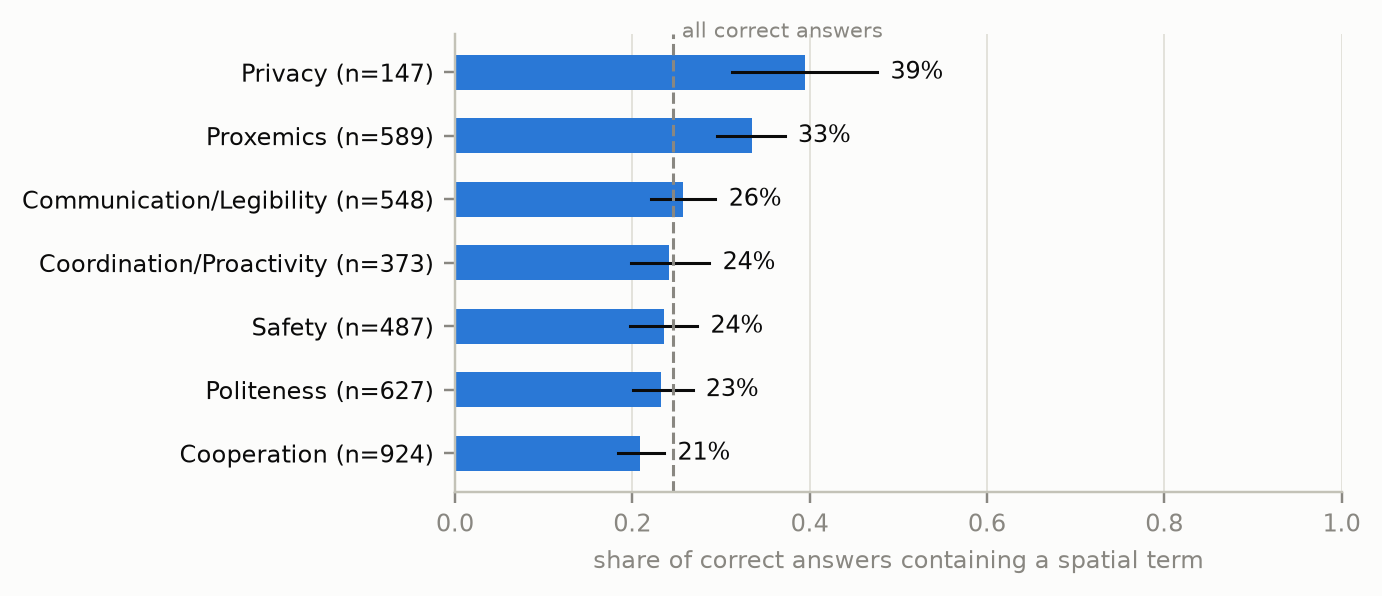
\includegraphics[width=\columnwidth]{spatial_language.png}
\caption{Share of correct answer options containing a spatial term, by norm category (categories overlap). Bars show 95\% bootstrap intervals; the dashed line is the rate over all correct options.}\label{fig:a3-spatial}
\end{figure}
\begin{figure}[h]\centering
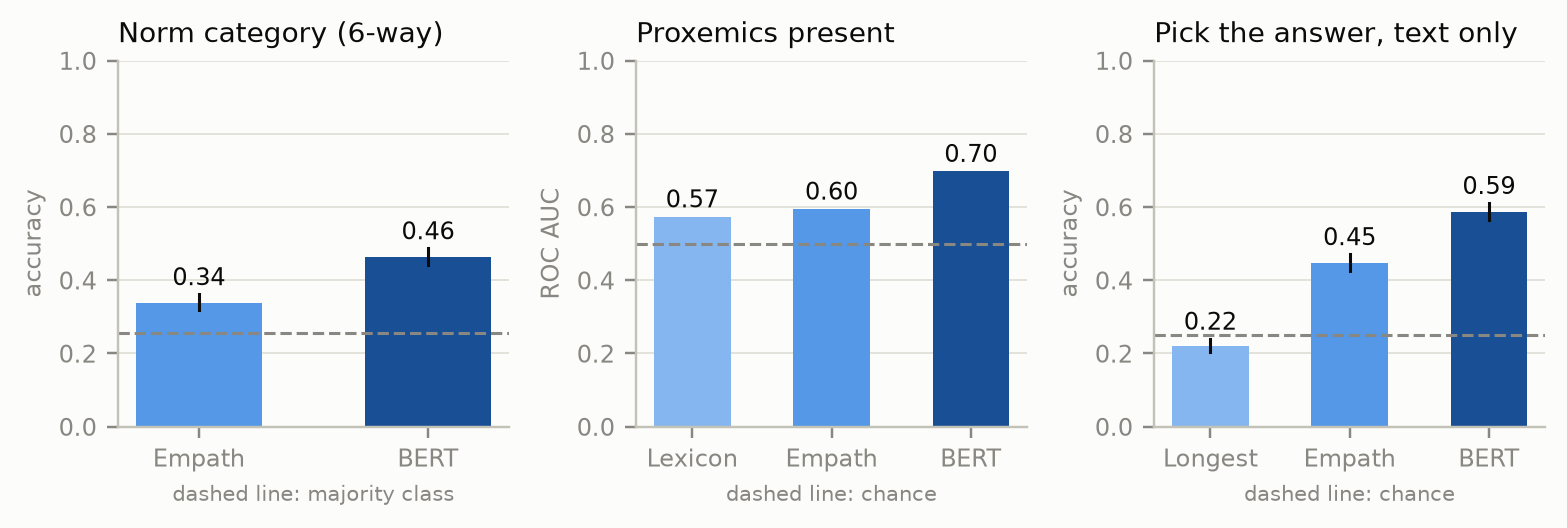
\includegraphics[width=\columnwidth]{representation_comparison.png}
\caption{Language representations on three label-related questions; folds grouped by source video.}\label{fig:a3-probe}
\end{figure}
\begin{figure}[h]\centering
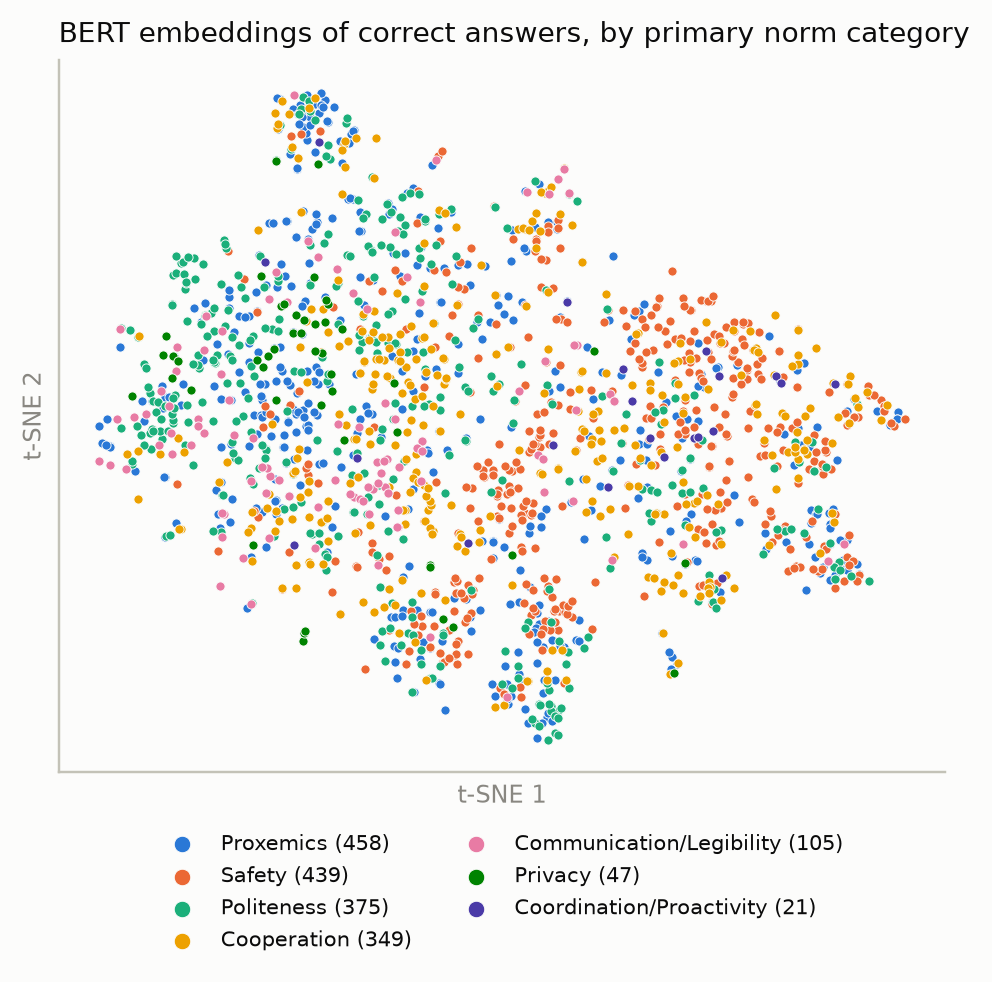
\includegraphics[width=0.85\columnwidth]{tsne_category.png}
\caption{t-SNE of BERT embeddings of correct options, coloured by primary norm category.}\label{fig:a3-tsne}
\end{figure}
